\documentclass[12pt,letterpaper]{article}
\usepackage{graphicx,textcomp}
\usepackage{natbib}
\usepackage{setspace}
\usepackage{fullpage}
\usepackage{color}
\usepackage[reqno]{amsmath}
\usepackage{amsthm}
\usepackage{fancyvrb}
\usepackage{amssymb,enumerate}
\usepackage[all]{xy}
\usepackage{endnotes}
\usepackage{lscape}
\newtheorem{com}{Comment}
\usepackage{float}
\usepackage{hyperref}
\newtheorem{lem} {Lemma}
\newtheorem{prop}{Proposition}
\newtheorem{thm}{Theorem}
\newtheorem{defn}{Definition}
\newtheorem{cor}{Corollary}
\newtheorem{obs}{Observation}
\usepackage[compact]{titlesec}
\usepackage{dcolumn}
\usepackage{tikz}
\usetikzlibrary{arrows}
\usepackage{multirow}
\usepackage{xcolor}
\newcolumntype{.}{D{.}{.}{-1}}
\newcolumntype{d}[1]{D{.}{.}{#1}}
\definecolor{light-gray}{gray}{0.65}
\usepackage{url}
\usepackage{listings}
\usepackage{color}

\definecolor{codegreen}{rgb}{0,0.6,0}
\definecolor{codegray}{rgb}{0.5,0.5,0.5}
\definecolor{codepurple}{rgb}{0.58,0,0.82}
\definecolor{backcolour}{rgb}{0.95,0.95,0.92}

\lstdefinestyle{mystyle}{
	backgroundcolor=\color{backcolour},   
	commentstyle=\color{codegreen},
	keywordstyle=\color{magenta},
	numberstyle=\tiny\color{codegray},
	stringstyle=\color{codepurple},
	basicstyle=\footnotesize,
	breakatwhitespace=false,         
	breaklines=true,                 
	captionpos=b,                    
	keepspaces=true,                 
	numbers=left,                    
	numbersep=5pt,                  
	showspaces=false,                
	showstringspaces=false,
	showtabs=false,                  
	tabsize=2
}
\lstset{style=mystyle}
\newcommand{\Sref}[1]{Section~\ref{#1}}
\newtheorem{hyp}{Hypothesis}

\title{Problem Set 2}
\date{October 14, 2024}
\author{Rafaela Alves}

\begin{document}
		\maketitle


	\section*{Question 1: Political Science}
		\vspace{.5cm}
	The following table was created using the data from a study run in a major Latin American city.\footnote{Fried, Lagunes, and Venkataramani (2010). ``Corruption and Inequality at the Crossroad: A Multimethod Study of Bribery and Discrimination in Latin America. \textit{Latin American Research Review}. 45 (1): 76-97.} As part of the experimental treatment in the study, one employee of the research team was chosen to make illegal left turns across traffic to draw the attention of the police officers on shift. Two employee drivers were upper class, two were lower class drivers, and the identity of the driver was randomly assigned per encounter. The researchers were interested in whether officers were more or less likely to solicit a bribe from drivers depending on their class (officers use phrases like, ``We can solve this the easy way'' to draw a bribe). The table below shows the resulting data.


\begin{table}[h!]
	\centering
	\begin{tabular}{l | c c c }
		& Not Stopped & Bribe requested & Stopped/given warning \\
		\\[-1.8ex] 
		\hline \\[-1.8ex]
		Upper class & 14 & 6 & 7 \\
		Lower class & 7 & 7 & 1 \\
		\hline
	\end{tabular}
\end{table}

\begin{enumerate}
	
	\item [(a)]
	Calculate the $\chi^2$ test statistic by hand/manually (even better if you can do "by hand" in \texttt{R}).\\

	
		\lstinputlisting[language=R, firstline=15, lastline=41]{PS02_myanswers_Rafaela.R}  
		
		Expected Frequency table:
		
		%pritning the table saved using stargazer
		
% Table created by stargazer v.5.2.3 by Marek Hlavac, Social Policy Institute. E-mail: marek.hlavac at gmail.com
% Date and time: Sun, Oct 13, 2024 - 18:44:42
\begin{table}[!htbp] \centering 
  \caption{} 
  \label{} 
\begin{tabular}{@{\extracolsep{5pt}} cccc} 
\\[-1.8ex]\hline 
\hline \\[-1.8ex] 
 & Not Stopped & Bribe Requested & Stopped/Given Warning \\ 
\hline \\[-1.8ex] 
Upper Class & $13.500$ & $8.357$ & $5.143$ \\ 
Lower Class & $7.500$ & $4.643$ & $2.857$ \\ 
\hline \\[-1.8ex] 
\end{tabular} 
\end{table} 

		
	
		x2 test statistic: \textbf{3.791168} 
		
		\vspace{0.5cm}
			
		Degrees of freedom: \textbf{2} 
	
		\vspace{0.5cm}
	
	\item [(b)]
	Now calculate the p-value from the test statistic you just created (in \texttt{R}).\footnote{Remember frequency should be $>$ 5 for all cells, but let's calculate the p-value here anyway.}  What do you conclude if $\alpha = 0.1$?\\
	
			\lstinputlisting[language=R, firstline=47, lastline=48]{PS02_myanswers_Rafaela.R}  
		
			\vspace{0.3cm}
			Conclusion:
			Since the p-value 0.150 is greater than $\sigma = 0.1$, it fails to reject the null hypothesis. This means there is not enough evidence to conclude that the class of the driver significantly affects whether a bribe is solicited or not.

\newpage

	\item [(c)] Calculate the standardized residuals for each cell and put them in the table below.
	\vspace{0.3cm}
	
		\lstinputlisting[language=R, firstline=59, lastline=70]{PS02_myanswers_Rafaela.R}  
	

	\begin{table}[h]
		\centering
		\begin{tabular}{l | c c c }
			& Not Stopped & Bribe requested & Stopped/given warning \\
			\\[-1.8ex] 
			\hline \\[-1.8ex]
			Upper class  & 0.136 & -0.815 & 0.818 \\
			\\
			Lower class & -0.182 & 1.093  & -1.098  \\
			
		\end{tabular}
	\end{table}
	
	
	\vspace{1cm}
	\item [(d)] How might the standardized residuals help you interpret the results?  
	\vspace{0.3cm}
	
	The largest standardized residual is in the "Bribe Requested" cell for lower-class drivers, with a value of 1.72. This suggests that lower-class drivers were more likely to be asked for bribes than we would expect under the null hypothesis of no relationship between class and outcome. On the other hand, upper-class drivers seem to have experienced a lower rate of bribe requests than expected. Thus, some deviation is visible for the "Stopped/Given Warning" category, but it's not as strong as the "Bribe Requested" result.
	
\end{enumerate}
\newpage

\section*{Question 2: Economics}
Chattopadhyay and Duflo were interested in whether women promote different policies than men.\footnote{Chattopadhyay and Duflo. (2004). ``Women as Policy Makers: Evidence from a Randomized Policy Experiment in India. \textit{Econometrica}. 72 (5), 1409-1443.} Answering this question with observational data is pretty difficult due to potential confounding problems (e.g. the districts that choose female politicians are likely to systematically differ in other aspects too). Hence, they exploit a randomized policy experiment in India, where since the mid-1990s, $\frac{1}{3}$ of village council heads have been randomly reserved for women. A subset of the data from West Bengal can be found at the following link: \url{https://raw.githubusercontent.com/kosukeimai/qss/master/PREDICTION/women.csv}\\

\noindent Each observation in the data set represents a village and there are two villages associated with one GP (i.e. a level of government is called "GP"). Figure~\ref{fig:women_desc} below shows the names and descriptions of the variables in the dataset. The authors hypothesize that female politicians are more likely to support policies female voters want. Researchers found that more women complain about the quality of drinking water than men. You need to estimate the effect of the reservation policy on the number of new or repaired drinking water facilities in the villages.
\vspace{.5cm}
\begin{figure}[h!]
	\caption{\footnotesize{Names and description of variables from Chattopadhyay and Duflo (2004).}}
	\vspace{.5cm}
	\centering
	\label{fig:women_desc}
	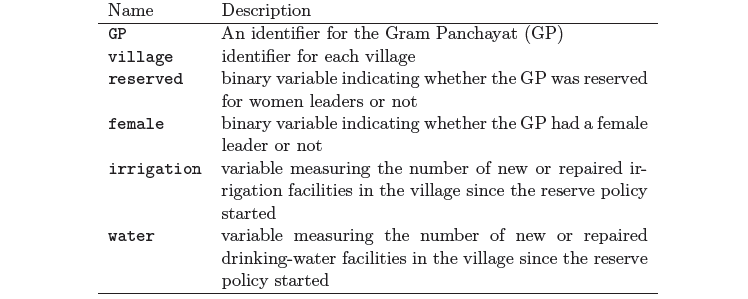
\includegraphics[width=1.1\textwidth]{women_desc.png}
\end{figure}		

\newpage
\begin{enumerate}
	\item [(a)] State a null and alternative (two-tailed) hypothesis. 
	\vspace{0.3cm}
	
	\textbf{Null Hypothesis:}
	The reservation policy does NOT have an effect on the number of new or repaired drinking water facilities in the villages. 
	\vspace{0.3cm}

	\textbf{Alternative Hypothesis:} 
	The reservation policy DOES have an effect on the number of new or 
	repaired drinking water facilities. 
	\vspace{1.2cm}
	
	
	
	\item [(b)] Run a bivariate regression to test this hypothesis in \texttt{R}.
		\vspace{0.3cm}
		
		For a bivariate regression in R to test the hypothesis, I'll regress the "water" variable on the "reserved" variable to check whether the reservation policy has an effect on the number of water facilities.
		\vspace{0.3cm}
	
		\lstinputlisting[language=R, firstline=113, lastline=119]{PS02_myanswers_Rafaela.R}  

	
	\begin{verbatim}
	Residuals:
	Min      1Q  Median      3Q     Max 
	-23.991 -14.738  -7.865   2.262 316.009 
	
	Coefficients:
	Estimate Std. Error t value Pr(>|t|)    
	(Intercept)   14.738      2.286   6.446 4.22e-10 ***
	reserved       9.252      3.948   2.344   0.0197 *  
	---
	Signif. codes:  0 ‘***’ 0.001 ‘**’ 0.01 ‘*’ 0.05 ‘.’ 0.1 ‘ ’ 1
	
	Residual standard error: 33.45 on 320 degrees of freedom
	Multiple R-squared:  0.01688,	Adjusted R-squared:  0.0138 
	F-statistic: 5.493 on 1 and 320 DF,  p-value: 0.0197
	\end{verbatim}
	
	\newpage
	
	\item [(c)] Interpret the coefficient estimate for reservation policy. 
	\vspace{0.3cm}
	
	The variable "reserved" has a coefficient of 7.564, which means that villages with reserved female leaders tend to have about 7.56 more drinking water facilities compared to those without reserved leaders. And considering the p-value (0.0136), we can reject the null-hypothesis and consider more evidences for the alternative-hypothesis that reservations with female leaderships do have more drinking water facilities. 
	
\end{enumerate}

\end{document}
